\chapter{Výběr konkrétního servomotoru}
\section{Požadavky na pohon}
\noindent\begin{minipage}{\textwidth}\centering
\resizebox{!}{48mm}{\begin{tikzpicture}[x=1cm,y=1cm]
% Pohled ve směru vodorovné osy hřídele; držák se pohybuje ve svislé rovině.
\fill[light] (-.7,-.8) rectangle (.7,.65);
\draw[thick] (-.7,-.8) rectangle (.7,.65);
\node[below,align=center] at (0,-.85) {MG996R\\pevně uchycené servo};
\draw[accent!60,dashed] (-3.3,0)--(0,0)--(0,3.3);
\draw[accent!60,dashed] (3.3,0) arc[start angle=0,end angle=180,radius=3.3];
\node[left] at (-3.3,0) {$180^\circ$};
\node[above] at (0,3.3) {$90^\circ$};
\node[right] at (3.95,0) {$0^\circ$};
\draw[accent,line width=4pt] (0,0)--(3.3,0);
\filldraw[fill=light,draw=accent,thick] (2.9,-.35) rectangle (3.7,.35);
\fill[ink] (3.3,0) circle (1.5pt);
\node[above right,align=left] at (3.8,.5) {Předmět na držáku\\$m=0{,}2\,\mathrm{kg}$};
\draw[thin] (3.65,.35)--(3.85,.5);
\filldraw[fill=white,draw=ink,thick] (0,0) circle (.15);
\fill[ink] (0,0) circle (1.5pt);
\draw[tok] (3.3,-.4)--(3.3,-1.65) node[right] {$F_g=mg$};
\draw[thin] (0,-.15)--(0,-.55);
\draw[thin] (3.3,-.4)--(3.3,-.55);
\draw[{Latex[length=1.5mm]}-{Latex[length=1.5mm]}] (0,-.48)--(3.3,-.48)
 node[midway,below] {$r=10\,\mathrm{cm}$};
\draw[tok,accent] (130:1.1) arc[start angle=130,end angle=35,radius=1.1];
\node[above right] at (.9,1.25) {Moment tíhy};
\node[align=left,anchor=west] at (4.2,2.2) {Rozsah držáku $0$--$180^\circ$\\ve svislé rovině};
\end{tikzpicture}
}
\captionsetup{hypcap=false}\captionof{figure}{Model držáku a jeho zatížení.}
\label{fig:drzak}
\end{minipage}

Držák se pohybuje ve svislé rovině; na obrázku je pohled ve směru hřídele. Vzdálenost $r$ vede k~těžišti zátěže. Ve vodorovné poloze je moment tíhy největší ($mgr$), nad osou nulový. Úhly je při montáži nutné sladit s~povelem serva.

Navrhujeme lehký polohovací držák s~rozsahem 0--180°. Příklad zatížení tvoří předmět o~hmotnosti \SI{0.2}{kg} ve vzdálenosti \SI{0.05}{m} od osy. V~nejméně příznivé vodorovné poloze vychází statický moment
\begin{equation}
 M=mgr=0{,}2\cdot9{,}81\cdot0{,}05\doteq\SI{0.098}{N.m}.
\end{equation}
Výpočet vychází z~modelové zátěže. Při realizaci přičteme hmotnost páky, tření a dynamický moment $J\alpha$. Změna mechanismu proto vyžaduje nový výpočet zatížení.

Moment se uvádí v~kgf\,cm, kde $1\,\mathrm{kgf\,cm}=\SI{0.0980665}{N.m}$. Katalogový moment při zablokování není dovolené trvalé zatížení; to bez tepelné charakteristiky nelze spolehlivě odvodit.

\section{Běžné modelářské servomotory}
Pro malé přípravky se často používají mikroserva SG90 a MG90S nebo větší MG996R. Liší se hlavně rozměry, převody a momentem. Tabulka porovnává katalogové údaje konkrétních provedení při stejném napětí 4,8 V; nejde o~dovolené trvalé zatížení.~\cite{sg90,mg90s,mg180}

\begin{table}[htbp]\centering\small
\caption{Srovnání běžných polohových RC serv při 4,8 V.}
\begin{tabularx}{\textwidth}{@{}lYYY@{}}\toprule
\textbf{Vlastnost} & \textbf{SG90 Digital} & \textbf{MG90S} & \textbf{MG996R 180°}\\\midrule
Hmotnost & 9 g & 13,4 g & 55 g\\\addlinespace
Převody & Plastové (POM) & Kovové & Kovové\\\addlinespace
Moment při zablokování & 1,8 kgf\,cm & 1,8 kgf\,cm & 9 kgf\,cm\\\addlinespace
Rychlost bez zatížení & 0,10 s/60° & 0,10 s/60° & 0,19 s/60°\\\addlinespace
Typické použití & Lehká klapka, model & Malý mechanismus s~odolnějšími převody & Větší držák, modelové rameno\\\bottomrule
\end{tabularx}
\end{table}

\FloatBarrier
\section{Zvolený model MG996R}
Pro držák volíme \textbf{MG996R s~kovovými převody v~polohovém provedení 180°}. Oproti mikroservům poskytuje větší momentovou rezervu. Parametry v~tabulce odpovídají zdokumentované 180° variantě; označení MG996R samo o~sobě nezaručuje stejné parametry všech prodávaných kusů.~\cite{mg180}

Moment 9 kgf\,cm odpovídá přibližně 0,88 N\,m, což je výrazně více než modelový požadavek 0,098 N\,m. Jde ale o~moment při zablokování, ze kterého nelze určit dovolené trvalé zatížení. Držák má být lehký a větší boční síly musí přenášet vlastní uložení. Přesnost omezují také vůle převodů.

\noindent\begin{minipage}{.67\textwidth}\small
\captionsetup{hypcap=false}\captionof{table}{Parametry MG996R 180°.~\cite{mg180}}
\begin{tabularx}{\linewidth}{@{}p{28mm}Y@{}}\toprule
\textbf{Parametr} & \textbf{Hodnota}\\\midrule
Napájení & 4,8--6 V\\
Moment při zablokování & 9 kgf\,cm (4,8 V); 11 kgf\,cm (6 V)\\
Rychlost bez zatížení & 0,19 s/60° (4,8 V); 0,18 s/60° (6 V)\\
Rozsah & 180°, polohové provedení\\
Rozměry & $40{,}7\times19{,}7\times42{,}9$ mm\\
Hmotnost & 55 g\\
Převody & Kovové\\\bottomrule
\end{tabularx}
\end{minipage}\hfill
\begin{minipage}{.29\textwidth}\centering
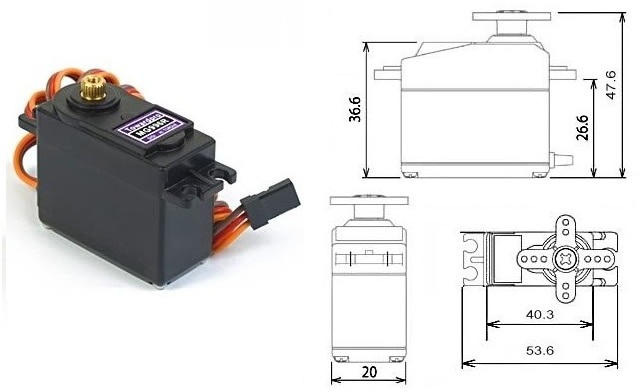
\includegraphics[trim=0 0 340 0,clip,width=\linewidth]{obrazky/foto/mg996r-datasheet.jpg}
\captionsetup{hypcap=false}\captionof{figure}{MG996R.~\cite{fotoMG996R}}
\end{minipage}\medskip

\section{Napájení a ověření rozsahu}
Samostatný katalogový list MG996R uvádí proud při zablokování 2,5 A~při 6 V, ale také jiné provedení s~rozsahem přibližně 120°. Proud proto použijeme jako předběžný návrhový odhad; údaje o~rozsahu nepřenášíme mezi variantami. Pro společné napájení serva a řízení volíme stabilizovaný zdroj 5 V / alespoň 4 A~a při realizaci ověříme skutečný odběr i napětí na konektoru.~\cite{mgpdf}

Pulzy 0,5--2,5 ms jsou návrhové meze generátoru, nikoli univerzální specifikace MG996R. Koncové polohy ověříme na konkrétním 180° kusu bez zatížení a bez tlačení do dorazů.
